% !TEX TS-program = pdflatex
% !TEX encoding = UTF-8 Unicode

\documentclass[a4paper]{article}

\usepackage[swedish]{babel}
\usepackage[T1]{fontenc}
\usepackage[utf8]{inputenc}
\usepackage[pdftex]{graphicx}
\usepackage{float}
\usepackage{fancyhdr}
\usepackage[toc,page]{appendix}
\usepackage{listings}
\usepackage{booktabs} % for much better looking tables
\usepackage{array} % for better arrays (eg matrices) in maths
\usepackage{paralist} % very flexible & customisable lists (eg. enumerate/itemize, etc.)
\usepackage{verbatim} % adds environment for commenting out blocks of text & for better verbatim
\usepackage{subfig} % make it possible to include more than one captioned figure/table in a single float

\def\changemargin#1#2{\list{}{\rightmargin#2\leftmargin#1}\item[]}
\let\endchangemargin=\endlist 

%%% HEADERS & FOOTERS
\author{Jonathan Karlsson, Niclas Olofsson, Paul Nedstrand\\jonka293, nicol, paune\\Grupp 2}
\pagestyle{fancy} % options: empty , plain , fancy
\renewcommand{\headrulewidth}{1pt} % customise the layout...
\fancyhead[LO,LE]{Jonathan, Niclas, Paul\\Rapport lab 2-3}
\lfoot{}\cfoot{\thepage}\rfoot{}

%%%% SECTION TITLE APPEARANCE
%\usepackage{sectsty}
%\allsectionsfont{\sffamily\mdseries\upshape} % (See the fntguide.pdf for font help)
%% (This matches ConTeXt defaults)
%
%%%% ToC (table of contents) APPEARANCE
%\usepackage[nottoc,notlof,notlot]{tocbibind} % Put the bibliography in the ToC
%\usepackage[titles,subfigure]{tocloft} % Alter the style of the Table of Contents
%\renewcommand{\cftsecfont}{\rmfamily\mdseries\upshape}
%\renewcommand{\cftsecpagefont}{\rmfamily\mdseries\upshape} % No bold!

%%% END Article customizations

%%% The "real" document content comes below...

\title{Rapport lab 2-3\\ \vspace{2 mm} {\large TSEA44}}
%\date{} % Activate to display a given date or no date (if empty),
         % otherwise the current date is printed 

\begin{document}
\maketitle

\newpage

\tableofcontents

\newpage
\section{Lab 1}
\subsection{Introduction}



Syftet med denna laboration var att konstruera en accelerator för jpeg-komprimering från raw-filer, i hårdvara. Detta löstes med hjälp av programmeringsspråket system verilog och genom att bygga vidare på det existerande skelettet som gavs med uppgiften. I första delen (labb2) så har vi en dator som styr själva acceleratorn och skickar all data via en bus för att sedan behandlas och lagras i ett blockminne där datorn sedan får läsa av resultatet. Ett register används för att starta grunkan och sedan läsa av att resultatet finns att hämta.
Det jpeg-acceleratorn gör är att ta ett block med 8x8 pixlar, skicka in det i en givet DCT maskin som gör komprimeringar av pixlarna, sedan transponeras de 8x8 pixlarna i ett minne och skickas tillbaka till DCT\rq{}n för att gå igenom en gång till. Alla pixlar multipliceras nu med hårdkodade reciprokaler och läggs i ett utminne. 
Datorn kan nu läsa av minnet, transponera och spara ner till en jpeg fil som kan öppnas på vanligt sätt.

\subsection{Implementation}



\begin{figure}[h]
\centering
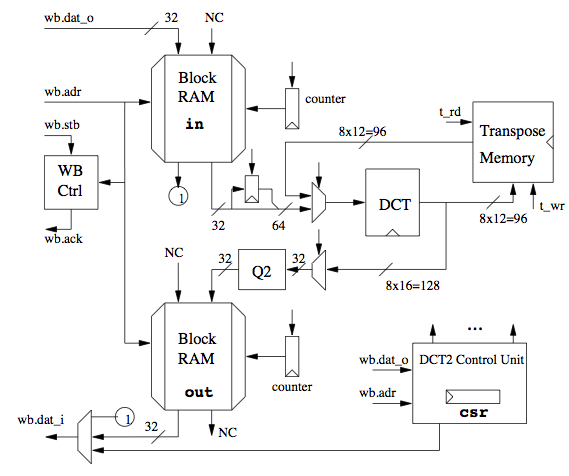
\includegraphics[scale=0.5]{architecture.png}
\caption{Arkitektur för vår design}
\label{fig:architecture}
\end{figure}


Figur \ref{fig:architecture} visar den arkitektur som konstruerades för att lösa uppgiften. All data som kommer in från bussen läggs in i minnet och vi väntar sedan på en startsignal från datorn. Då används räknaren tillsammans med en vippa för att skicka in data till DCT\rq{}n för att sedan skriva in 8x8 pixlar till transponeringsminnet, när vi skrivit klart där så läser vi av kolumnerna (och får därigenom transponeringen), skickar in till DCT\rq{}n igen.

Ett problem vi hade så här långt var klockningen, när vi skickar in data från inminnet så måste vi göra det 8 pixlar åt gången, men i minnet finns bara 4 pixlar per rad, så vi måste läsa två rader (därav vippan), vidare måste vi klocka ner DCT\rq{}n en klockcykel för att den ska \lq\lq{}hinna med\rq\rq{}. Läsningen från transponeringen var inget problem, däremot när pixlarna kommer ut den andra gången måste klockningen anpassas till Q2-maskinen då den tar två pixlar per klockcykel så DCT\rq{}n måste gå ytterligare långsammare för att detta ska fungera.

\begin{figure}[h]
\centering
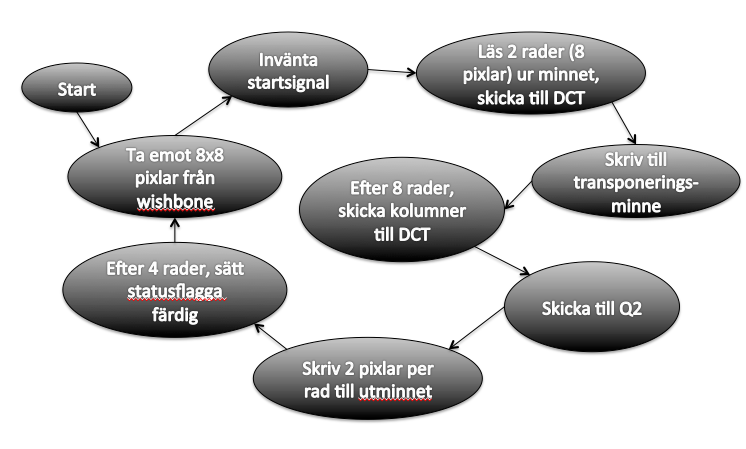
\includegraphics[width=340px]{states.png}
\caption{Tillståndsgraf för vår design}
\label{fig:state}
\end{figure}
Figur \ref{fig:state} visar en tillståndsgraf över maskinen och dess procedur för att komprimera raw-filer till jpeg. Tillståndsgrafen följer precis det schema som arkitekturen i figur \ref{fig:architecture} också visar.

\subsection{Vidare frågor}


\section{Labb 3}
\subsection{Introduktion}
Designen från labb 2 visas i figur \ref{fig:architecture} och innebär att datorn måste engagera sig en hel del och en stor flaskhals för prestandan ligger i bussen som används. Dels måste datorn läsa ur alla pixlar från minnet, via bussen, sedan skicka iväg pixlarna igen via bussen till jpeg-acceleratorn för att sedan skicka en startsignal för varje 8x8 pixlar. När acceleratorn är färdig måste datorn läsa av det i ett register varpå datorn läser av minnet i acceleratorn och skickar ännu mer pixlar genom bussen. 

Den flaskhalsen skulle man kunna spara in en del på genom att acceleratorn själv hämtar sin data från minnet istället för att gå genom datorn, där gör den ändå ingen nytta. Så idén är att ha en ytterligare design som hämtar data och skickar in till acceleratorn, sätter igång den självmant. Datorn måste fortfarande läsa av registret för att kontrollera att acceleratorn är färdig samt hämta de färdiga pixlarna, men bussen besparas ändå en hel del data med denna lösning.

\subsection{Design}


\section{Resultat}

\subsection{Prestanda}

\begin{table}[ht]
    \centering
    \begin{tabular}{l l}
    
        Beskrivning & Antal klockcykler\\
        \hline
        Main program  & 33 902 171 \\
        Init  &  9 850 924 \\
        Encode\_image  & 24 051 247 \\
        Forward\_DCT  & 8 317 191 \\
        Copy  & 1 518 825 \\
        DCT kernel  & 0 \\
        Quantization  & 6 798 366 \\
        Huffman encoding  & 15 246 407 \\
        Emit\_bits  &  7 904 811 \\
    \end{tabular}
    \caption{ Prestanda för JPEG-acceleratorn }
    \label{tab:jpeg_performance_2}
\end{table}

\subsection{FPGA-användning}
\begin{table}[ht]
    \centering
    \begin{tabular}{l l l}
        Flip Flops   &      7 273 out of   46080  & 15\% \\
        4 input LUTs &      11 485 out of  46080  & 24\% \\
        MULT18X18s   &      19 out of 120  &   15\% \\
        RAMB16s      &      42 out of 120  &   35\% \\
    \end{tabular}
    \caption{ De mest intressanta delarna ur syntes-rapporten för JPEG-acceleratorn med DCT, DMA samt sbit-instruktionen. }
    \label{tab:fpga_usage}
\end{table}
%Logic Utilization:
%  Total Number Slice Registers:       7,305 out of  46,080   15%
%    Number used as Flip Flops:        7,273
%    Number used as Latches:              32
%  Number of 4 input LUTs:            11,485 out of  46,080   24%
%Logic Distribution:
%  Number of occupied Slices:          8,264 out of  23,040   35%
%    Number of Slices containing only related logic:   8,264 out of   8,264 100%
%    Number of Slices containing unrelated logic:          0 out of   8,264   0%
%      *See NOTES below for an explanation of the effects of unrelated logic.
%  Total Number of 4 input LUTs:      11,742 out of  46,080   25%
%    Number used as logic:            11,317
%    Number used as a route-thru:        257
%    Number used for Dual Port RAMs:     168
%      (Two LUTs used per Dual Port RAM)
%  Number of bonded IOBs:                217 out of     824   26%
%    IOB Flip Flops:                     246
%  Number of RAMB16s:                     42 out of     120   35%
%  Number of MULT18X18s:                  19 out of     120   15%
%  Number of BUFGMUXs:                     5 out of      16   31%
%  Number of DCMs:                         2 out of      12   16%
%
%labb2 :::
%Performance statistics:
%Cycles spent in main program: 33902171
%+-- Cycles spent in init: 9850924
%+-- Cycles spent in encode_image: 24051247
%+-- Cycles spent in forward_DCT: 8317191
%| +-- Cycles spent in copy: 1518825
%| +-- Cycles spent in DCT kernel: 0
%| +-- Cycles spent in quantization: 6798366
%+-- Cycles spent in Huffman encoding: 15246407
%+-- Cycles spent in emit_bits: 7904811
%
%
%
%Device Utilization Summary:
%
%Number of BUFGMUXs 5 out of 16 31%
%Number of DCMs 2 out of 12 16%
%Number of External IOBs 217 out of 824 26%
%Number of LOCed IOBs 217 out of 217 100%
%
%Number of MULT18X18s 19 out of 120 15%
%Number of RAMB16s 42 out of 120 35%
%Number of LOCed RAMB16s 12 out of 42 28%
%
%Number of SLICEs 8264 out of 23040 35%
%
%
%labb3 ::: 
%Performance statistics:
%Cycles spent in main program:             25847242
%+-- Cycles spent in init:                  6600044
%+-- Cycles spent in encode_image:         19247198
%    +-- Cycles spent in forward_DCT:       6489189
%    |   +-- Cycles spent in copy:                0
%    |   +-- Cycles spent in DCT kernel:          0
%    |   +-- Cycles spent in quantization:  6489189
%    +-- Cycles spent in Huffman encoding: 12226950
%        +-- Cycles spent in emit_bits:     4983905
%
%
%Device Utilization Summary:
%
%Number of BUFGMUXs 5 out of 16 31%
%Number of DCMs 2 out of 12 16%
%Number of External IOBs 217 out of 824 26%
%Number of LOCed IOBs 217 out of 217 100%
%
%Number of MULT18X18s 19 out of 120 15%
%Number of RAMB16s 42 out of 120 35%
%Number of LOCed RAMB16s 12 out of 42 28%
%
%Number of SLICEs 8604 out of 23040 37%



\section{Sammanfattning}



\subsection{Filer}
\begin{itemize}
	\item [jpegtop.sv] Mestadels av designen skedde här, våra kontrollsignaler ligger här tillsammans med flera räknare och minnen.
	\item [transpose.sv] Transponeringsminnet fick en egen fil med en kolumnräknare och en radräknare för att hålla koll på vart grunkan håller på att läsa respektive skriva.
	\item [q2.sv] Denna sköter multipliceringen med reciprokalerna och skickar sedan resultatet till utminnet.
	\item [jpegdma.sv] Designen för den andra biten där jpeg-acceleratorn själv läser av informationen i minnet.
\end{itemize}


\section{What to Include in the Lab Report 2}
\begin{itemize}
\item How did you verify that your 2D DCT hardware works correctly?
\item Isthesizeofthe2DDCThardwarejustifiedbytheperformanceimprovements?
\item What would be required in order to implement more functionality like zigzag addressing in the 2D DCT hardware module? Would it be difficult to modify jpegfiles to take advantage of such optimizations?
And of course, the normal parts of a lab report such as a table of contents, an intro- duction, a conclusion, etc. The source code that you have written should be included in appendices and referred to from the main document.
\end{itemize}


\section{What to Include in the Lab Report 3}
The lab report should contain all source code that you have written. (The source code should of course be commented.) We would also like you to include a block diagram of your hardware. If you have written any FSM you should include a state diagram graph of the FSM.
We would also like you to discuss the following questions in detail somewhere in your lab report1:
\begin{itemize}
\item How does your hardware work?
\item How did you verify that your hardware worked?
\item How did you modify the software?
\item A timing diagram.
\item What is the utilization of your accelerator?
\item What is the performance of jpegtest with DMA enabled?
\item How long does it take (on average) to read a macroblock into the DCT acceler- ator via DMA?
\item How much is the wishbone bus used by the DMA unit and how much is the bus used by the CPU?
And of course, the normal parts of a lab report such as a table of contents, an intro- duction, a conclusion, etc. The source code that you have written should be included in appendices and referred to from the main document.
\end{itemize}





\newpage
\begin{appendices}
\begin{changemargin}{-3cm}{-3cm} 
\section{jpegtop.sv}
\lstinputlisting[language=Verilog,caption={Kod för labb 2},label=jpeg_top]{jpeg_top.sv}

\section{transpose.sv}
\lstinputlisting[language=Verilog,caption={Kod för transponeringen},label=selection-sort]{transpose.sv}

\section{Q2.sv}
\lstinputlisting[language=Verilog,caption={Kod för kvantiseringen},label=q2]{q2.sv}

\section{jpegdma.sv}
\lstinputlisting[language=Verilog,caption={Kod för labb 3},label=jpeg_dma]{jpeg_dma.sv}
\end{changemargin}
\end{appendices}


\end{document}
